%%%%%%%% ICML 2026 submission: Cross-Size KV Handoff %%%%%%%%
% Text converted from docs/paper-eeai-draft-2026-09-22.md; numbers from
% analysis/cloud/summary.md. Figures: docs/paper/make_figs.py.
% Build: latexmk -pdf main.tex   (from docs/paper/)

\documentclass{article}

\usepackage{microtype}
\usepackage{graphicx}
\usepackage{subcaption}
\usepackage{booktabs}
\usepackage{hyperref}
\newcommand{\theHalgorithm}{\arabic{algorithm}}

% Blind submission version. For a preprint use \usepackage[preprint]{icml2026};
% for camera-ready use \usepackage[accepted]{icml2026}.
\usepackage{icml2026}

\usepackage{amsmath}
\usepackage{amssymb}
\usepackage{mathtools}
\usepackage[capitalize,noabbrev]{cleveref}
\usepackage{multirow}

\graphicspath{{figs/}}

\icmltitlerunning{Cross-Size KV Handoff}

\begin{document}

\twocolumn[
  \icmltitle{Cross-Size KV Handoff: A Small Model's Cache \\ Can Be Read by a Larger One}

  % Anonymous author block (double-blind submission).
  \icmlsetsymbol{equal}{*}
  \begin{icmlauthorlist}
    \icmlauthor{Anonymous Authors}{anon}
  \end{icmlauthorlist}
  \icmlaffiliation{anon}{Anonymous Institution, Anonymous City, Anonymous Country}
  \icmlcorrespondingauthor{Anonymous Author}{anon.email@domain.com}
  \icmlkeywords{KV cache, latent communication, model handoff, multi-agent LLM}

  \vskip 0.3in
]

\printAffiliationsAndNotice{}

\begin{abstract}
Agents built from several language models hand work to each other through text, which drops everything the sender computed while reading. We ask whether a smaller model's key--value (KV) cache can be handed directly to a larger model of the same family. Between K2-Horizon-3.7B and K2-Horizon-7B, a per-head linear map fit in closed form recovers almost nothing (22\% on a binding test, chance 12.5\%), but a gated residual on top of it, trained for 1,500 steps on the larger model's continuation loss with both models frozen, lets the 7B answer 63--73\% of questions about facts only the 3.7B read. Three controls separate content from compute: a cache from the wrong episode drops accuracy to 5\% and the 7B follows the wrong cache 64\% of the time; a projector trained with a deranged sender learns a soft prompt that recovers 77\% of the continuation-loss gap yet answers at 23\%; and injecting the cache into only the first half of the receiver's layers gives chance, while the second half alone gives 52\%. Transfer does not degrade when the fact is 512 tokens away from the question and holds across three attribute types. We release the maps and the test.
\end{abstract}

\section{Introduction}
\label{sec:intro}

Edge--cloud agent stacks run a small model on device and escalate to a large one when the small model is unsure. Escalation today means re-sending the transcript: the large model re-reads everything and the small model's work is discarded. If the large model could instead continue from the small model's internal state, the handoff would carry what the small model had already computed---including, in the longer run, how sure it was.

This paper asks the narrowest version of that question. Given two frozen models of different size that share a tokenizer and KV geometry (K2-Horizon-3.7B and 7B: 36 layers, 8 KV heads, head dimension 128), can a learned map from the small model's cache to the large model's cache carry a \emph{specific fact} that only the small model saw? We call this binding transfer, and we test it with a control for the standard objection that ``latent gains'' are extra compute rather than communication.

\textbf{Contributions.}
(1) A binding-transfer test (Noma) with six arms that isolates content from shape and compute.
(2) A two-stage projector---closed-form ridge over correlation-selected source layers, plus a gated residual trained on the receiver's continuation loss---that reaches 63--73\% binding transfer where the ridge alone reaches 22\%.
(3) Three controls that bound what the receiver actually gets from the cache: a deranged-episode cache, a deranged-sender projector, and layer-band injection.

\section{Setup}
\label{sec:setup}

\textbf{Models.} Sender K2-Horizon-3.7B, receiver K2-Horizon-7B, both frozen, bf16, RoPE $\theta = 10^{7}$. We capture the sender's pre-RoPE K and raw V at every layer, map them, apply RoPE at the receiver, and insert the result as the receiver's cache for the prefix positions. The receiver then reads only the question.

\textbf{Projector.} Stage 1: for each receiver layer $\ell$ and KV head $h$, a ridge regression from the concatenated $[K;V]$ of the sender (256-d per head) to the receiver's $[K;V]$; source layers are the three sender layers whose K/V correlate best with receiver layer $\ell$ (``top-3''), which beat the aligned-layer map in a first pass. Stage 2: a gated SwiGLU residual (bottleneck 128, ${\sim}150$M parameters) on top of the ridge output, trained with AdamW for 1,500 steps, effective batch 16 sequences of 1,024 FineWeb-Edu tokens, prefix 512, on the receiver's cross-entropy over the continuation. Nothing in training mentions the test.

\textbf{Noma binding test.} Each episode assigns one of eight single-token values to eight nonce names (``Noma is amber. Vela is indigo.\ \ldots''). Only the sender reads the facts. The receiver is asked ``What colour is Vela?'' and we score the eight values. Arms: \emph{none} (question only), \emph{text} (receiver reads the facts itself), \emph{self} (receiver's own cache re-injected; equals \emph{text} to $10^{-4}$), \emph{raw} (sender cache injected without a map), \emph{project} (mapped cache), \emph{derange} (mapped cache from another episode with the same layout but a different value for the queried name). Content transfer $=$ project $-$ derange. For \emph{derange} we also report the follow rate: how often the answer is the \emph{other} episode's value.

\section{Results}
\label{sec:results}

\begin{table}[t]
\caption{Binding transfer, 8 names $\times$ 8 values, $n = 1000$ episodes, chance 12.5\%. All entries are percentages. ``follow'' is the rate at which the receiver, handed the deranged cache, answers with the other episode's value; ``content'' is project $-$ derange.}
\label{tab:main}
\vskip 0.1in
\begin{center}
\begin{small}
\resizebox{\columnwidth}{!}{%
\begin{tabular}{lccccccc}
\toprule
projector & none & text & raw & project & derange & follow & content \\
\midrule
ridge top-3 (closed form)          & 10.6 & 100 & 14 & 21.7 & 11.4 & 18.2 & 10.3 \\
$+$ residual, 1500 steps           & 10.6 & 100 & 14 & \textbf{63.0} & 4.6 & \textbf{63.7} & 58.4 \\
residual, deranged sender          & 10.6 & 100 & 14 & 23.4 & 11.3 & 22.7 & 12.1 \\
\bottomrule
\end{tabular}}
\end{small}
\end{center}
\vskip -0.1in
\end{table}

\begin{figure}[t]
\centering
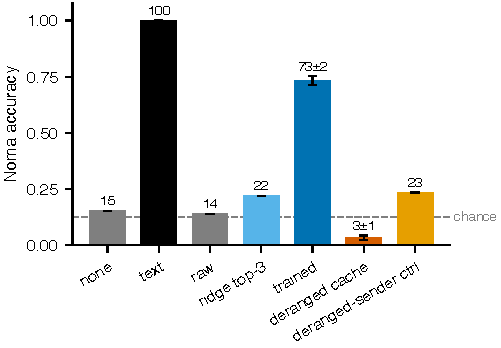
\includegraphics[width=\columnwidth]{fig_arms.pdf}
\caption{Noma accuracy by arm on the 6-name variant ($n = 300$). ``trained'' and ``deranged cache'' are the mean over three training seeds with error bars showing one standard deviation; the deranged-sender control is the \emph{project} arm of the projector trained with a deranged sender ($n = 1000$, 8-name variant). Dashed line: chance (12.5\%).}
\label{fig:arms}
\end{figure}

\Cref{tab:main} and \cref{fig:arms} give the main result. On the original 6-name variant ($n = 300$) three training seeds give 71.3 / 73.0 / 75.3\% (mean 73.2, sd 2.0). Two ablations on the same variant: freezing the ridge and training only the residual gives 59.0\%, so letting the linear map move during training is worth ${\sim}14$ points; replacing the correlation-selected top-3 source layers with the aligned-layer map gives 32.7\%, so which sender layers feed each receiver layer is the single largest design choice. Matching shape alone (\emph{raw}) does nothing. The follow rate is the decisive number: when the receiver is handed the wrong episode's cache it answers with the wrong episode's value 64\% of the time, and its accuracy falls below chance. The receiver believes the cache.

With the full 8-name pool and 500 episodes, the seed-2 projector gives 65.8\% and 67.6\% on two episode seeds (ridge: 20.4\%, 20.6\%). On 256 fresh held-out sequences deduplicated against training text, continuation retention is 1.19 for the trained projector and $-0.38$ for the ridge.

\textbf{Other attributes.} Same protocol with cities (``Vela lives in Paris'') and animals (``Vela is a fox''), $n = 500$: trained projector 61.8\% and 67.2\%; ridge 19.8\% and 12.8\%; deranged-sender control 15.4\% and 12.4\%.

\begin{figure}[t]
\centering
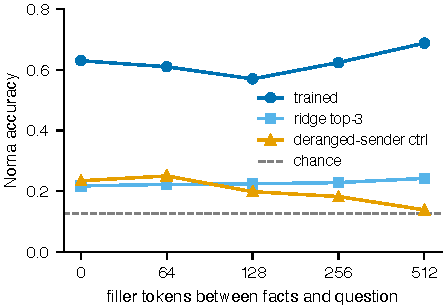
\includegraphics[width=\columnwidth]{fig_distance.pdf}
\caption{Noma accuracy as a function of the number of neutral filler tokens between the facts and the question (8-name variant; $n = 1000$ at 0, $n = 500$ otherwise). Transfer does not decay with distance; the best value is at the training prefix length of 512.}
\label{fig:distance}
\end{figure}

\textbf{Distance.} Padding the facts with neutral filler so the question is 64 / 128 / 256 / 512 tokens after them: 61.0 / 57.0 / 62.4 / 68.8\% (\cref{fig:distance}). No decay; the best value is at the training prefix length.

\begin{table}[t]
\caption{Where the binding lives. This episode's mapped cache is injected only into a band of receiver layers, the deranged episode's elsewhere. $n = 500$, 6-name variant; accuracy in percent.}
\label{tab:layers}
\vskip 0.1in
\begin{center}
\begin{footnotesize}
\setlength{\tabcolsep}{3pt}
\begin{tabular}{lcccccccc}
\toprule
layers   & 0--5 & 0--11 & 0--17 & 12--23 & 24--35 & 30--35 & 18--35 & all \\
\midrule
accuracy & 7.2 & 8.0 & 10.4 & 28.6 & 30.8 & 7.6 & 51.8 & 63.0 \\
\bottomrule
\end{tabular}
\end{footnotesize}
\end{center}
\vskip -0.1in
\end{table}

\begin{figure}[t]
\centering
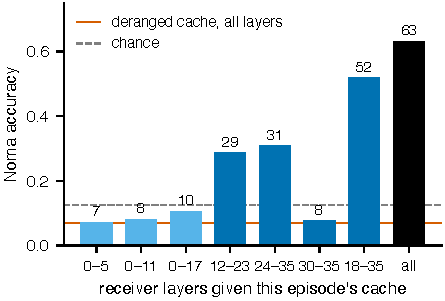
\includegraphics[width=\columnwidth]{fig_layers.pdf}
\caption{Noma accuracy when only the labelled band of receiver layers receives this episode's mapped cache (the deranged episode's cache fills the rest). Solid line: the deranged cache in all layers; dashed line: chance.}
\label{fig:layers}
\end{figure}

\textbf{Where the binding lives.} \Cref{tab:layers} and \cref{fig:layers}: the first half of the network carries nothing usable on its own; the second half alone carries most of it, and no six-layer band suffices. The binding is read out from a distributed set of later layers.

\begin{table}[t]
\caption{Real passages: SQuAD v1.1 validation. The sender reads the passage ($\le 512$ tokens); the receiver reads only the question and answers greedily ($\le 8$ tokens, stopped at newline). Token-F1 against the gold spans, $n = 300$ (600 for the trained projector); mean gold log-probability per token.}
\label{tab:qa}
\vskip 0.1in
\begin{center}
\begin{small}
\resizebox{\columnwidth}{!}{%
\begin{tabular}{lccccccc}
\toprule
receiver sees & none & text & raw & ridge & trained & \shortstack{deranged-\\sender ctrl} & \shortstack{trained,\\derange arm} \\
\midrule
F1 & 16.6 & 54.7 & 0.6 & 14.3 & \textbf{53.0}\,(51.8) & 15.1 & 13.8 \\
gold log-prob / token & $-3.57$ & $-0.90$ & $-11.2$ & $-3.88$ & $-1.74$ & $-3.77$ & $-4.18$ \\
\bottomrule
\end{tabular}}
\end{small}
\end{center}
\vskip -0.1in
\end{table}

\begin{figure}[t]
\centering
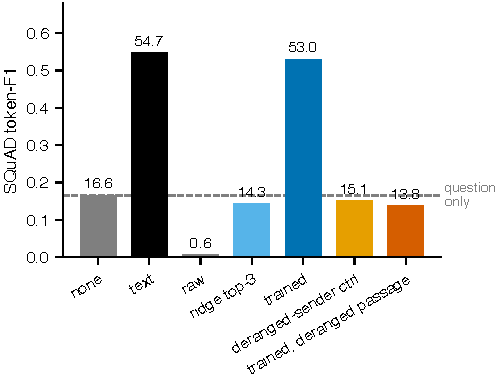
\includegraphics[width=\columnwidth]{fig_qa.pdf}
\caption{SQuAD token-F1 by arm ($n = 300$). Dashed line: question only. The trained projector sits within two points of the receiver reading the passage itself; the ridge map, the deranged-sender control, and the trained projector given the wrong passage's cache all sit at or below question-only.}
\label{fig:qa}
\end{figure}

\textbf{Real passages.} \Cref{tab:qa} and \cref{fig:qa} apply the same projectors, never trained on questions, to SQuAD v1.1. On F1 the trained projector recovers 96\% of the gap between question-only and reading the passage (53.0 at $n = 300$; 51.8 at $n = 600$); on gold log-probability it recovers 69\%. The wrong passage's cache (derange), the ridge map, and the content-free projector all sit at or below question-only. The channel carries the passage, not a bias toward answering.

\section{Controls}
\label{sec:controls}

Three controls bound what the receiver actually gets from the cache.

\textbf{Deranged cache.} The \emph{derange} arm of \cref{tab:main}: a mapped cache from another episode with the same layout but a different value for the queried name. Accuracy falls to 4.6\% and the receiver answers with the other episode's value 63.7\% of the time. The receiver is not ignoring the cache; it is reading it.

\textbf{Deranged-sender projector.} A projector trained with the identical recipe but with the sender reading text unrelated to the receiver's continuation. It cannot learn a content channel, only a soft prompt. It reaches 23.4\% on the binding test (\cref{tab:main}, row 3) and 15.1 F1 on SQuAD (\cref{tab:qa}), both at the question-only level.

\begin{table}[t]
\caption{Continuation retention is the wrong headline. Retention $= (\mathrm{loss}_{\text{none}} - \mathrm{loss}_{\text{project}}) / (\mathrm{loss}_{\text{none}} - \mathrm{loss}_{\text{oracle}})$ on 128 fresh held-out sequences; the second column swaps the sender's text at test time.}
\label{tab:retention}
\vskip 0.1in
\begin{center}
\begin{small}
\begin{tabular}{lcc}
\toprule
projector & retention & \shortstack{retention, sender\\text deranged} \\
\midrule
ridge top-3                          & $-0.30$ & $-0.66$ \\
$+$ residual                         & 1.23    & 0.31 \\
residual, deranged sender & 0.77    & 0.72 \\
\bottomrule
\end{tabular}
\end{small}
\end{center}
\vskip -0.1in
\end{table}

\begin{figure*}[t]
\centering
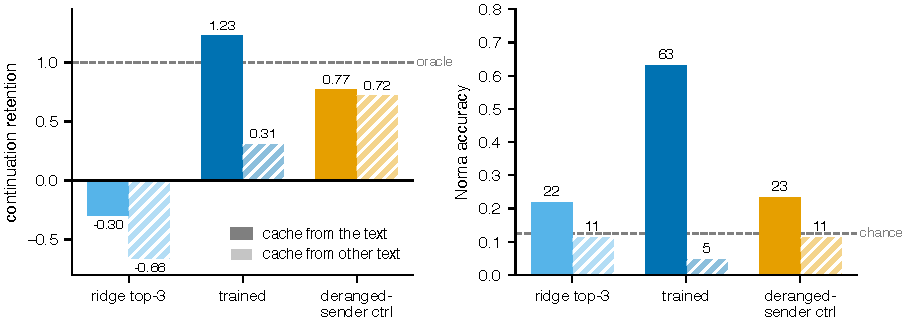
\includegraphics[width=\textwidth]{fig_retention.pdf}
\caption{Retention and the binding test disagree about the deranged-sender control. Left: continuation retention on 128 fresh held-out sequences for the three projectors, with the sender reading the true prefix (solid) or a swapped one (hatched). Right: Noma accuracy for the same three projectors ($n = 1000$, 8-name variant), \emph{project} arm (solid) and \emph{derange} arm (hatched). Retention ranks the content-free projector at 0.77, most of which survives a swapped sender; the binding test puts it at chance.}
\label{fig:retention}
\end{figure*}

\textbf{Continuation retention is the wrong headline.} Following the closed-form-map literature \citep{2608.03893} we also report retention (\cref{tab:retention}, \cref{fig:retention}). A projector trained with the sender reading the \emph{wrong} text---a learned soft prompt with no content channel---recovers 77\% of the oracle gap, and almost all of it (0.72) survives when its input is deranged at test time. The trained projector's 1.23 decomposes into ${\sim}0.3$ of the same prompt-like effect and ${\sim}0.9$ that disappears when the sender's text is swapped. Retention above 1 is therefore not evidence of communication, and retention alone cannot distinguish a channel from a prompt; the binding test with its derange arm can.

\textbf{Layer-band injection.} \Cref{tab:layers} and \cref{fig:layers}, discussed above: injecting this episode's cache into layers 0--17 alone gives chance (10.4\%); layers 18--35 alone give 51.8\%; no six-layer band suffices.

\section{Related Work}
\label{sec:related}

Cache-to-cache communication \citep[C2C;][]{2510.03215} and Latent Cache Flow \citep{2605.22863} train fusers between models of similar size; a closed-form KV map \citep{2608.03893} reports 44--98\% continuation retention across sizes; a causal audit \citep{2608.04893} finds that deranged caches lose only 0.4 points in such setups, which is the objection our derange and deranged-sender arms answer. A second audit \citep{2607.26773} decomposes the aggregate effect of a latent channel into ``sender content'' and ``any message present'' terms with boundary-replacement controls; our deranged-sender projector isolates the second term directly. Dual-Cache \citep{2608.20617}, CacheBridge \citep{2609.00891} and HyLaT \citep{2605.25421} extend cache transfer to heterogeneous pairs and hybrid latent--text protocols. The Replay Gap \citep{2608.08239} and Confidence Laundering \citep{2606.20662} argue that handoffs must be evaluated on branched rollouts and must carry uncertainty; both are next steps for this line. These works are concurrent with ours; we treat them as the surrounding conversation, not as prior results this paper improves on.

\section{Limitations}
\label{sec:limitations}

The results show that a specific fact can cross from a 3.7B cache into a 7B without text, that the crossing depends on the cache's content, and that the receiver reads it out from its later layers. They do not show that the channel is cheaper than text (a 512-token cache is ${\sim}75$\,MB against ${\sim}1$\,KB of text; compression is future work), that it carries anything richer than a single-token binding, or that it works across model families. The channel is not one-way: with the roles swapped (7B sender, 3.7B receiver, same recipe) the ridge map gives 29.0\% and the trained projector 63.3\% on the 6-name test, with the deranged cache at 5.7\% and a 63\% follow rate---the same pattern at slightly lower accuracy. All results are on a single model family and a single size pair.

\section{Conclusion}
\label{sec:conclusion}

A learned cache map turns a size-mismatched pair of frozen models into a sender and a receiver. The controls matter more than the headline: the wrong cache is followed, the content-free projector fails the test, and the signal is read out late in the receiver. The next question is whether the same channel can carry how sure the sender was.

\section*{Impact Statement}

This paper presents work whose goal is to advance the field of machine learning. There are many potential societal consequences of our work, none of which we feel must be specifically highlighted here. One consideration specific to cache handoff: a cache that a receiver ``believes'' (\cref{sec:controls}) is also a cache that can be tampered with; deployments that move caches between devices should authenticate them as they would any other input.

\bibliography{refs}
\bibliographystyle{icml2026}

\newpage
\appendix
\onecolumn

\section{Ablations on the 6-Name Variant}
\label{app:ablations}

All runs: sender K2-Horizon-3.7B, receiver K2-Horizon-7B, colour attribute, 6 names, $n = 300$ episodes, chance 12.5\%. Accuracy in percent.

\begin{table}[h]
\caption{Projector ablations on the 6-name Noma variant.}
\label{tab:ablations}
\vskip 0.1in
\begin{center}
\begin{small}
\begin{tabular}{lccc}
\toprule
projector & project & derange & follow \\
\midrule
ridge top-3 (closed form)                     & 22.0 & 10.7 & 30.3 \\
$+$ residual, 300 steps                       & 56.3 & 6.3  & 53.7 \\
$+$ residual, 1500 steps, seed 0              & 71.3 & 4.3  & 71.7 \\
$+$ residual, 1500 steps, seed 1              & 73.0 & 3.0  & 74.0 \\
$+$ residual, 1500 steps, seed 2              & 75.3 & 2.3  & 76.0 \\
$+$ residual, 1500 steps, ridge frozen        & 59.0 & 7.0  & 59.3 \\
$+$ residual, 1500 steps, aligned-layer ridge & 32.7 & 8.0  & 34.7 \\
\bottomrule
\end{tabular}
\end{small}
\end{center}
\end{table}

\section{Other Attributes and Reversed Roles}
\label{app:attrs}

\begin{table}[h]
\caption{Binding transfer with city and animal attributes ($n = 500$, 8 names) and with the roles reversed (7B sender, 3.7B receiver; 6 names, $n = 300$).}
\label{tab:attrs}
\vskip 0.1in
\begin{center}
\begin{small}
\begin{tabular}{llcccc}
\toprule
setting & projector & none & project & derange & follow \\
\midrule
city   & ridge top-3            & 14.2 & 19.8 & 11.8 & 18.4 \\
city   & trained                & 14.2 & 61.8 & 6.4  & 60.2 \\
city   & deranged-sender ctrl   & 14.2 & 15.4 & 11.4 & 18.6 \\
animal & ridge top-3            & 12.2 & 12.8 & 12.0 & 11.2 \\
animal & trained                & 12.2 & 67.2 & 5.2  & 64.6 \\
animal & deranged-sender ctrl   & 12.2 & 12.4 & 12.8 & 9.8 \\
reversed & ridge top-3          & 11.7 & 29.0 & 12.3 & 31.3 \\
reversed & trained              & 11.7 & 63.3 & 5.7  & 63.0 \\
\bottomrule
\end{tabular}
\end{small}
\end{center}
\end{table}

\section{Distance Sweep}
\label{app:distance}

\begin{table}[h]
\caption{Noma accuracy (\emph{project} arm) versus filler tokens between facts and question. 8-name variant; $n = 1000$ at pad 0, $n = 500$ otherwise.}
\label{tab:distance}
\vskip 0.1in
\begin{center}
\begin{small}
\begin{tabular}{lccccc}
\toprule
projector & 0 & 64 & 128 & 256 & 512 \\
\midrule
ridge top-3          & 21.7 & 22.2 & 22.4 & 22.8 & 24.2 \\
trained              & 63.0 & 61.0 & 57.0 & 62.4 & 68.8 \\
deranged-sender ctrl & 23.4 & 25.0 & 19.8 & 18.2 & 13.8 \\
\bottomrule
\end{tabular}
\end{small}
\end{center}
\end{table}

\end{document}
